
\documentclass{beamer}

\usepackage[german]{babel}
\usepackage[utf8]{inputenc}
\usepackage{pdfpages}
\usepackage{color}
\usepackage{graphicx, import}
\usepackage{amsmath}
\usepackage{amssymb}
\usepackage{amsthm}
\usepackage[percent]{overpic}
\usepackage{tikz}
\usepackage{mathtools}
\usepackage[font=footnotesize, justification=centering]{caption}
\usepackage{subcaption}


\usetheme{CambridgeUS}
\setbeamertemplate{enumerate items}[default]

%\newtheorem{definition}{Definition}
\newtheorem{thm}{Satz}
%\newtheorem{lemma}{Lemma}

\makeatletter
\def\input@path{{../../images/}}
\makeatother

\renewcommand{\proofname}{Beweis}
\captionsetup{font=small, justification=centering}
\graphicspath{{../../images/}}
\addto\captionsgerman{\renewcommand{\figurename}{}} % name figures 'Abb.' (change it for babel)

\title[Distanzerhaltende Approximation]{Distanzerhaltende Approximation von Kantenzügen}
\author[N. Klug]{Nikolas Klug}
\institute[Uni Augburg]{Universität Augsburg}
\date{17. Mai 2018}


\begin{document}
	\frame{\titlepage}
	
	\section{Einführung in die Problemstellung}
	\begin{frame}

		\begin{figure}
			\includegraphics<1>[height=0.8\textheight]{maps_zoom4.png}
			\includegraphics<2>[height=0.8\textheight]{maps_zoom3.png}
			\includegraphics<3>[height=0.8\textheight]{maps_zoom2.png}
			\includegraphics<4>[height=0.8\textheight]{maps_zoom1_red_box.png}

			\caption{\tiny{Grenze zwischen Deutschland und Österreich. Quelle: \emph{Google Maps}, Stand 8. Mai 2018, \href{https://www.google.de/maps/@47.5869372,11.6674982,9.06z}{https://www.google.de/maps/@47.5869372,11.6674982,9.06z}}}
		\end{figure}
		
	\end{frame}
	
	\begin{frame}{Definition Kantenzug}

		\centering
		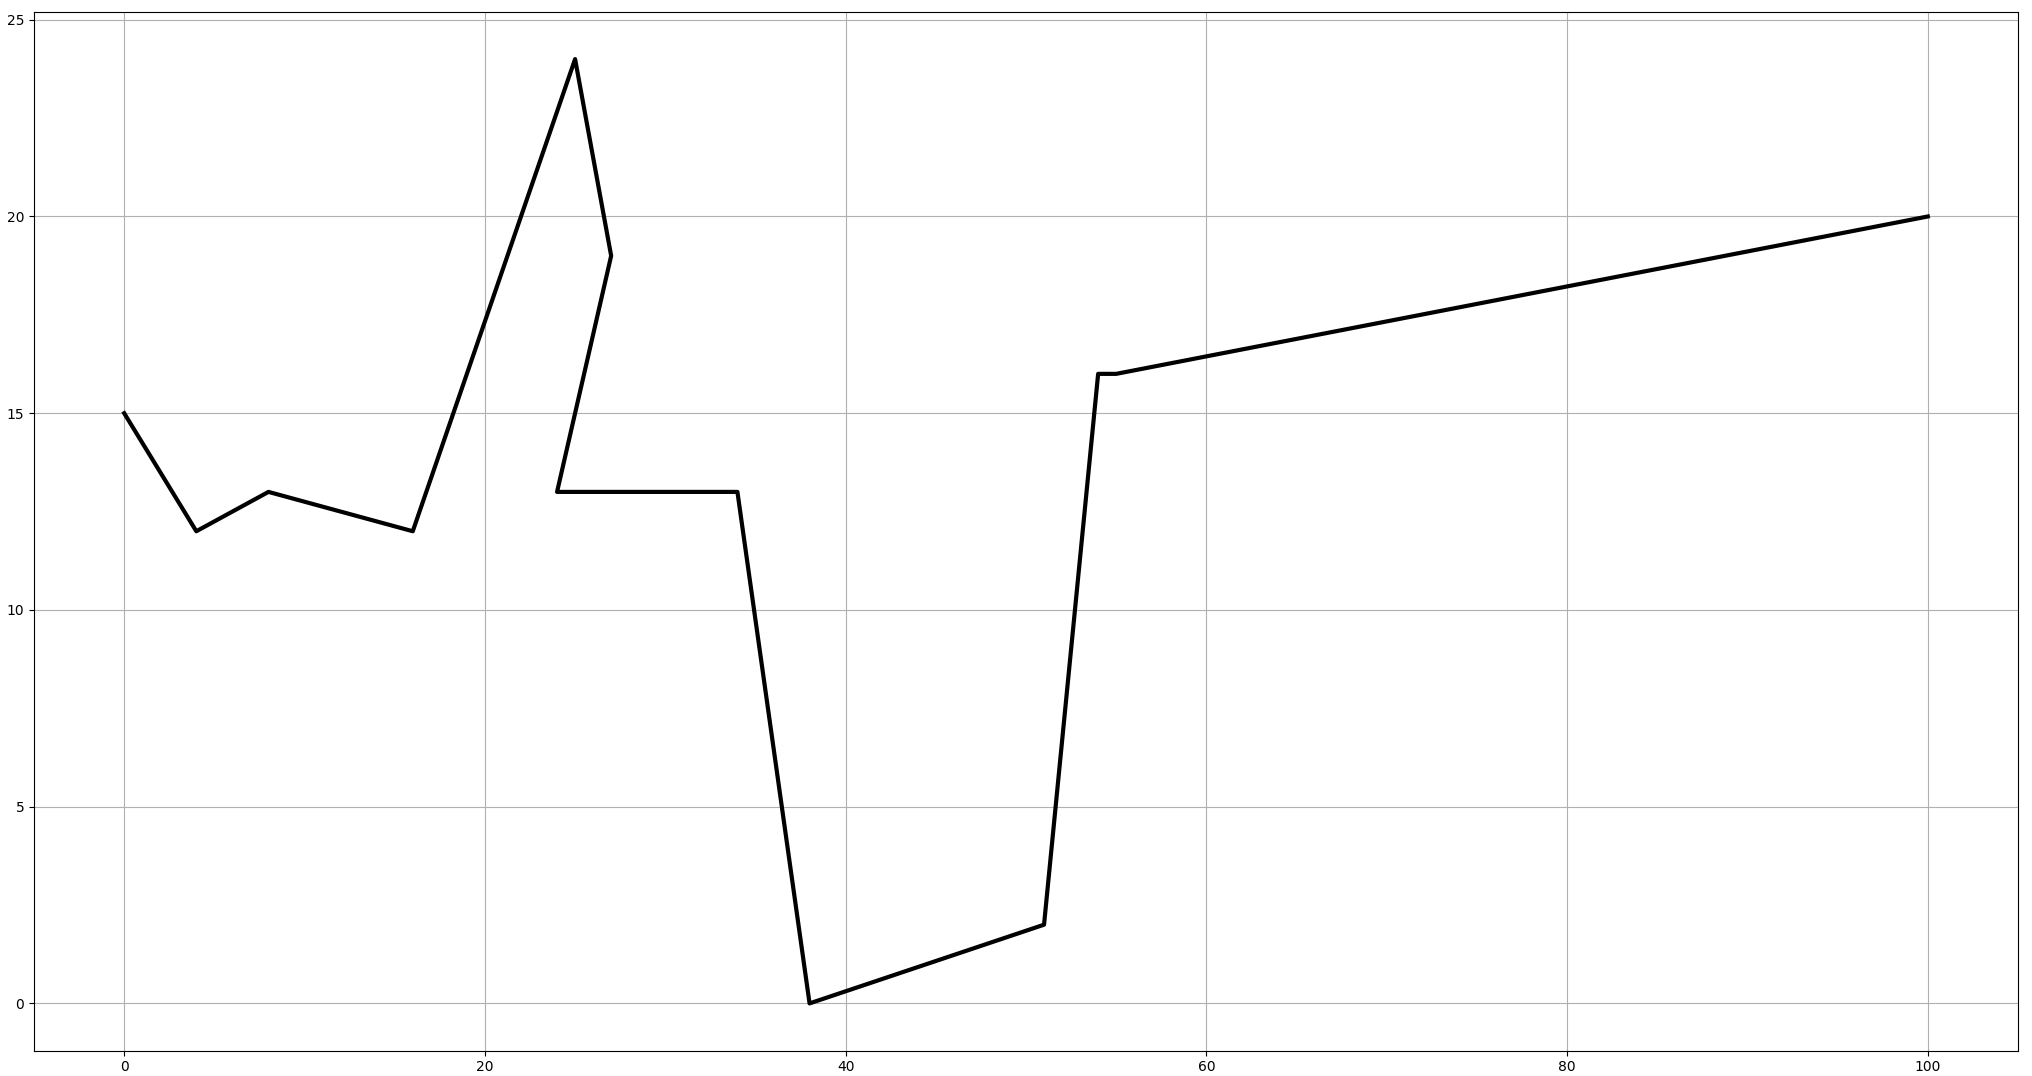
\includegraphics[height=0.6\textheight]{raw_path.png}
		
		\begin{definition}
			Sei $n, d \in \mathbb{N}$ und für $1 \leq i \leq n$ $p_i \in \mathbb{R}^d$.
			Ein \emph{(polygonaler) Kantenzug} $P = (p_1, p_2, \mathellipsis, p_n)$ ist eine Aneinanderreihung von Geradensegmenten, die für $1 \leq i < n$ jeweils die Punkte $p_i$ und $p_{i+1}$ verbinden. 

		\end{definition}
	\end{frame}
	
	\begin{frame}{Definition $t$-distanzerhaltend}
		Sei $P = (p_1, \mathellipsis, p_n)$ ein Kantenzug und $p_i, p_j \in P$.
		\begin{itemize}
			\item<1-> $|p_ip_j|$ ist die euklidische Distanz zwischen $p_i$ und $p_j$.
			\item<2->$\delta(p_i, p_j)~\coloneqq~\sum\limits_{k=i}^{j-1}{|p_kp_{k+1}|}$ ist die Distanz entlang des Pfades.
		\end{itemize}
		\begin{definition}<3->
			Seien $t \in \mathbb{R}$, $t \geq 1$ und $p_i, p_j \in P$. 
			Dann ist die Kante $(p_i, p_j)$ genau dann \emph{$t$-distanzerhaltend}, wenn $\delta(p_i, p_j) \leq t \cdot |p_ip_j|$.
		\end{definition}
		
	\end{frame}
	
	\begin{frame}
		\centering
		$(p_i, p_j)$ \emph{$t$-distanzerhaltend} $\Leftrightarrow$ $\delta(p_i, p_j) \leq t \cdot |p_ip_j|$.
		\vspace{0.5cm}
		\begin{figure}
			\centering
			\begin{subfigure}{.5\textwidth}
				\centering
				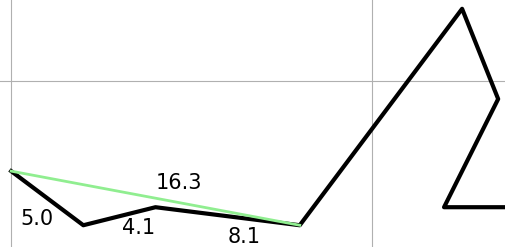
\includegraphics[width=0.95\linewidth]{t_distance_preserving_edge_len.png}
				\caption{$t$-distanzerhaltend}

			\end{subfigure}%
			\begin{subfigure}{.5\textwidth}
				\centering
				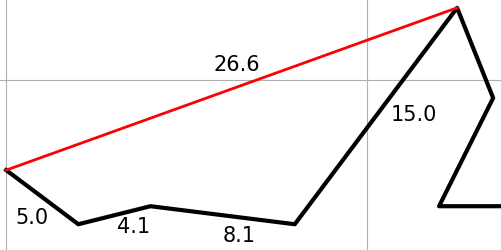
\includegraphics[width=0.95\linewidth]{not_t_distance_preserving_edge_len.png}
				\caption{nicht $t$-distanzerhaltend}
			\end{subfigure}
			\caption{ (nicht) $t$-distanzerhaltende Kanten für $t = 1.2$}
		\end{figure}
	\end{frame}
	
	\begin{frame}{Definition $t$-distanzerhaltende Approximation}
		\begin{definition}
			Ein Kantenzug $Q = (p_{i_1}, p_{i_2}, \mathellipsis, p_{i_k})$ ist genau dann eine \emph{$t$-distanzerhaltende Approximation von $P = (p_1, p_2, \mathellipsis, p_n)$}, wenn beide der folgenden Bedingungen gelten.
			\begin{enumerate}
				\item $\displaystyle 1 = i_1 < i_2 < \mathellipsis < i_k = n$.
				\item $\displaystyle \text{Für alle } 1 \leq l < k \text{ ist die Kante } (p_{i_l}, p_{i_{l+1}})$ des Kantenzugs $t$-distanzerhaltend.
			\end{enumerate}
		\end{definition}
		\begin{figure}
			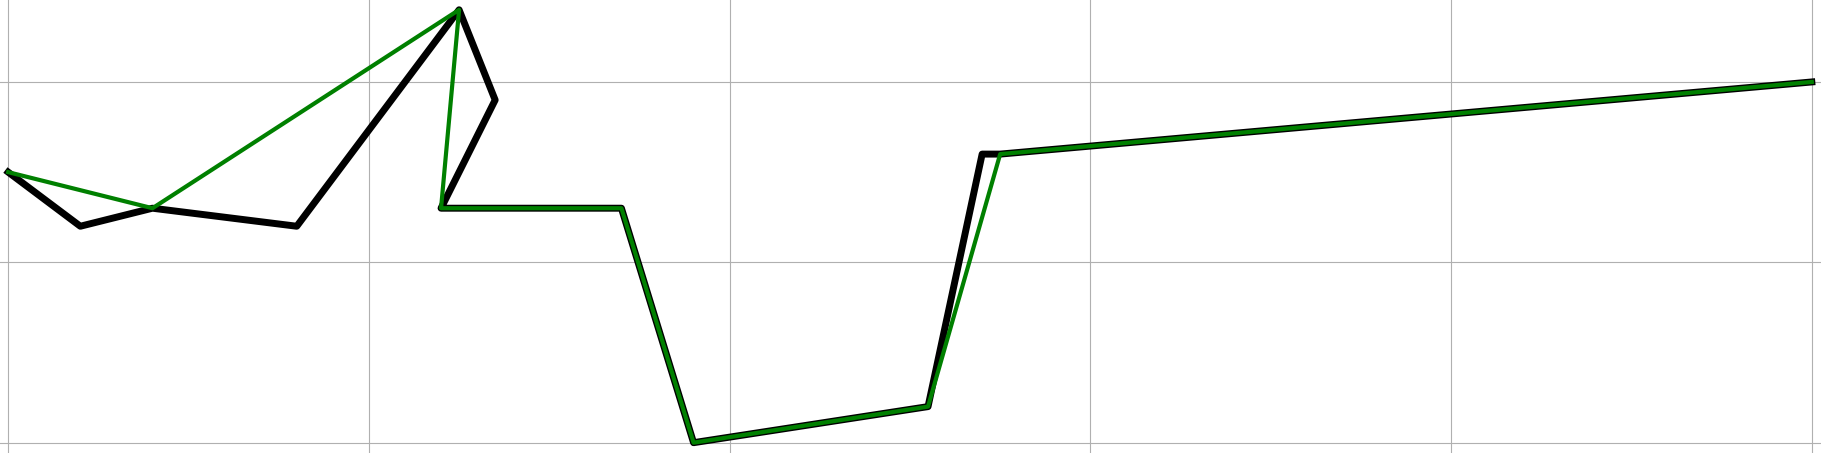
\includegraphics[width=\textwidth]{approximation_example.png}
		\end{figure}
	\end{frame}
	
	\begin{frame}{Problemspezifikation}
		\begin{definition}[Minimum-Vertex-Path-Simplification]
			Liegt ein polygonaler Kantenzug $P$ und eine reelle Zahl $t \geq 1$ vor, soll eine minimale $t$-distanzerhaltende Approximation von $P$ berechnet werden.
		\end{definition}
		\begin{definition}[Minimum-Dilation-Path-Simplification]
			Liegt ein polygonaler Kantenzug $P$ und eine natürliche Zahl $k$ vor, soll der kleinste Wert $t$ bestimmt werden, für den eine $t$-distanzerhaltende Approximation von $P$ mit maximal $k$ Knoten existiert.
		\end{definition}

	\end{frame}
	
	\section{Exakte Algorithmen}
	\subsection{MVPS}
	\begin{frame}{Exakter Algorithmus für das MVPS-Problem}
		Sei $P = (p_1, p_2, \mathellipsis, p_n)$ ein Kantenzug und $t \geq 1$.
		\begin{description}
			\item[Schritt 1:]<1-> Konstruktion des gerichteten Graphen $G_t = (V, E_t)$, wobei:
			\begin{itemize}
				\setlength{\itemindent}{-1.3cm}
				\item $V = \{p_1, \mathellipsis, p_n\}$
				\item $E_t = \{(p_i, p_j) \in V\times V|\ i < j\ \text{und}\ (p_i,p_j)\ \text{ist $t$-distanzerhaltend}\}$
			\end{itemize}
			\item[Schritt 2:]<3-> Bestimmen eines kürzesten Pfades in $G_t$ von $p_1$ nach $p_n$
		\end{description}
		\uncover<2->{
			\begin{figure}
				\begin{overprint}
					\onslide<2-3>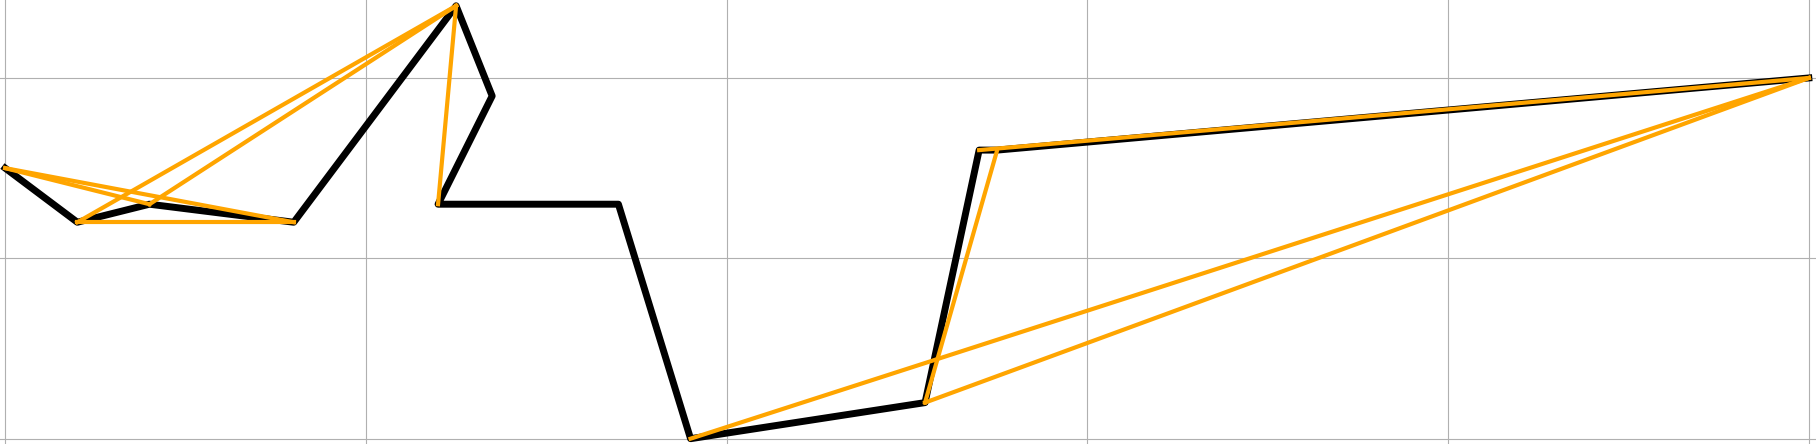
\includegraphics[width=\textwidth]{path_t_distance_preserving_edges_cropped.png}
					\onslide<4->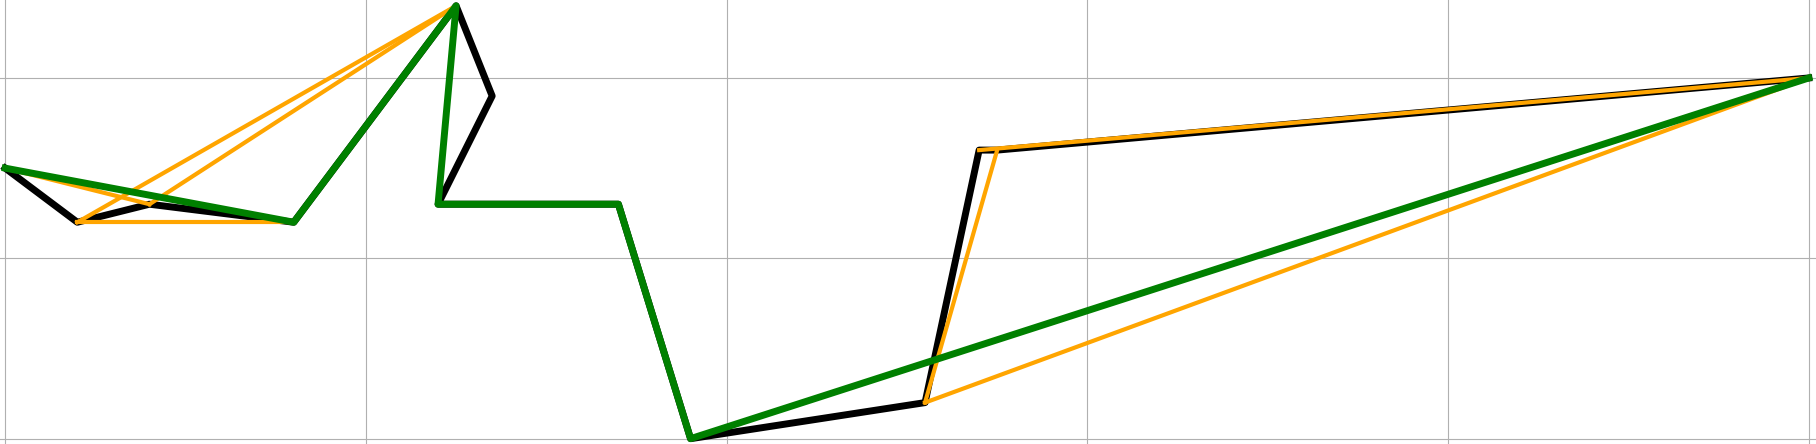
\includegraphics[width=\textwidth]{shortest_path_with_t_edges.png}
				\end{overprint}
				\begin{overprint}
					\onslide<2-3>\caption{$G_t$ für $t = 1.2$}
					\onslide<4->\caption{Kürzester Pfad in $G_t$}
				\end{overprint}
			\end{figure}}
	\end{frame}
	
	\begin{frame}{Laufzeit}
		\begin{columns}
			\begin{column}{0.6\linewidth}
				\begin{description}
					\item[Schritt 1:]<1-> Konstruktion des Graphen $G_t$
					\item[Schritt 2:]<2-> Breitensuche
				\end{description}
			\end{column}
			\begin{column}{0.5\linewidth}
				\begin{description}
					\item[]<1-> $O(n^2)$
					\item[]<2-> $O(n + m) = O(n^2)$
				\end{description}
			\end{column}
		\end{columns}
		\begin{thm}<3->
			Das Minimum-Vertex-Path-Simplification Problem kann für Kantenzüge mit $n$ Knoten in $O(n^2)$ Zeit gelöst werden.
		\end{thm}
	\end{frame}
	
	\subsection{MDPS}
	\begin{frame}{Exakter Algorithmus für das MDPS-Problem}
		Sei $P = (p_1, \mathellipsis, p_n)$ und $k$ die gewünschte Knotenzahl.
		
		Sei $\kappa_t$ die Knotenzahl einer minimalen $t$-distanzerhaltenden Approximation von $P$.
		
		\begin{lemma}
			Sind $t, t' \in \mathbb{R}$ und $1 \leq t < t'$, dann ist $\kappa_t \geq \kappa_{t'}$.
		\end{lemma}
		\textit{Beweis.}
			\begin{itemize}
				\item[] Annahme: $\kappa_{t} < \kappa_{t'}$.
				
				\item[$\Leftrightarrow$]Eine minimale $t$-distanzerhaltende Approximation von $P$ hat echt weniger Knoten als eine minimale $t'$-distanzerhaltende. 
				
				\item[] Aber: Jede $t$-distanzerhaltende Approximation von $P$ ist auch eine $t'$-distanzerhaltende Approximation von $P$.
				
				Das ist ein Widerspruch.
			\end{itemize}
			
	\end{frame}
	
	\begin{frame}[t]{Exakter Algorithmus für das MDPS-Problem}
			\begin{lemma}
				Sind $t, t' \in \mathbb{R}$ und $1 \leq t < t'$, dann ist $\kappa_t \geq \kappa_{t'}$.
			\end{lemma}
			Sei $t^*$ die Lösung des Problems.
			
			$t^*_{ij} \coloneqq \frac{\delta(p_i, p_j)}{|p_ip_j|}$ heißt \emph{Abweichung} der Kante $(p_i, p_j)$ vom Kantenzug.
			\vspace{10px}
		\begin{description}
			\item[Schritt 1:]<1-> Berechnen von $M \coloneqq \{t^*_{ij}\ |\ 1\leq i < j \leq n\}$
			\item[Schritt 2:]<2-> Sortieren von $M$
			\item[Schritt 3:]<3-> Binäre Suche im $M$ nach $t^*$:
			\begin{itemize}
				\setlength{\itemindent}{-1.3cm}
				\item Lösen des MVPS-Problems für den aktuellen $t$-Wert.
				\item Sei $\kappa_t$ die Knotenzahl der Lösung. 
				Falls $\kappa_t \leq k$, so ist $t \geq t^*$.
				Sonst ist $\kappa_t > k$ und somit $t < t^*$.
			\end{itemize}
		\end{description}
	\end{frame}
	
	\begin{frame}{Laufzeit}
		\begin{columns}
			\begin{column}{0.5\textwidth}
				\begin{description}
					\item[Schritt 1:]<1-> Berechnen von $M$
					\item[Schritt 2:]<2-> Sortieren von $M$
					\item[Schritt 3:]<3-> Binäre Suche
				\end{description}
			\end{column}
			\begin{column}{0.6\textwidth}
				\begin{description}
					\item[]<1-> $O(n^2)$
					\item[]<2-> $O(n^2 \log n^2) = O(n^2 \log n)$
					\item[]<3-> $O(n^2 \log n^2) = O(n^2 \log n)$
				\end{description}
			\end{column}
		\end{columns}
		\begin{thm}<3->
			Das Minimum-Dilation-Path-Simplification Problem kann für Kantenzüge mit $n$ Knoten in $O(n^2 \log n)$ Zeit gelöst werden.
		\end{thm}
	\end{frame}
	
	\section{Approximativer Algorithmus für das MVPS-Problem}
	\subsection{WSPD}
	\begin{frame}{Definition wohl-separiert}
		Seien $s > 0$ und $A$ und $B$ zwei endliche Mengen von Punkten in $\mathbb{R}^d$. 
		\begin{definition}
			$A$ und $B$ heißen \emph{wohl-separiert bezüglich $s$}, falls es zwei disjunkte Bälle $C_A$ und $C_B$ gibt, die denselben Radius $R$ haben, sodass $A \subseteq C_A$ und $B \subseteq C_B$ und die euklidische Distanz zwischen den Rändern von $C_A$ und $C_B$ mindestens $s\cdot R$ beträgt.
		\end{definition}
		\uncover<2-3>{\begin{figure}
			\centering
			\alt<2>{
				\def\svgwidth{\textwidth}
				\input{well_separated_2D.pdf_tex}
			}{
				\def\svgwidth{\textwidth}
				\small{\input{well_separated_1D.pdf_tex}}

			}
		\end{figure}}
	\end{frame}
	
	\begin{frame}{Definition WSPD}
		\begin{definition}
			\label{def:wspd}
			Sei $S \subseteq \mathbb{R}^d$ und $s > 0$. 
			Eine Menge $ \{(A_1, B_1), (A_2, B_2), \mathellipsis, (A_m, B_m)\}$ von Paaren von nicht-leeren Teilmengen von $S$ ist genau dann eine \emph{Zerlegung in wohl-separierte Paare}, wenn für alle $1 \leq i \leq m$ gilt:
			\begin{enumerate}
				\item $A_i \cap B_i = \emptyset$.
				\item Für alle $p, q \in S$ gibt es genau einen Index $1 \leq j \leq m$, sodass entweder $p \in A_j$ und $q \in B_j$ oder $q \in A_j$ und $p \in B_j$.
				\item $A_i$ und $B_i$ sind bezüglich $s$ wohl-separiert.
			\end{enumerate}
		\end{definition}
	\end{frame}
	
	\begin{frame}{WSPD - Algorithmus für unsere Anwendung}
		\begin{itemize}
			\item Transformation des Eingabekantenzuges $P = (p_1, p_2, \mathellipsis, p_n)$ auf eine eindimensionale Folge $S = (x_1, x_2, \mathellipsis, x_n)$, wobei $x_i = \delta(p_1, p_i)$
		\end{itemize}
		\begin{figure}
			\centering
			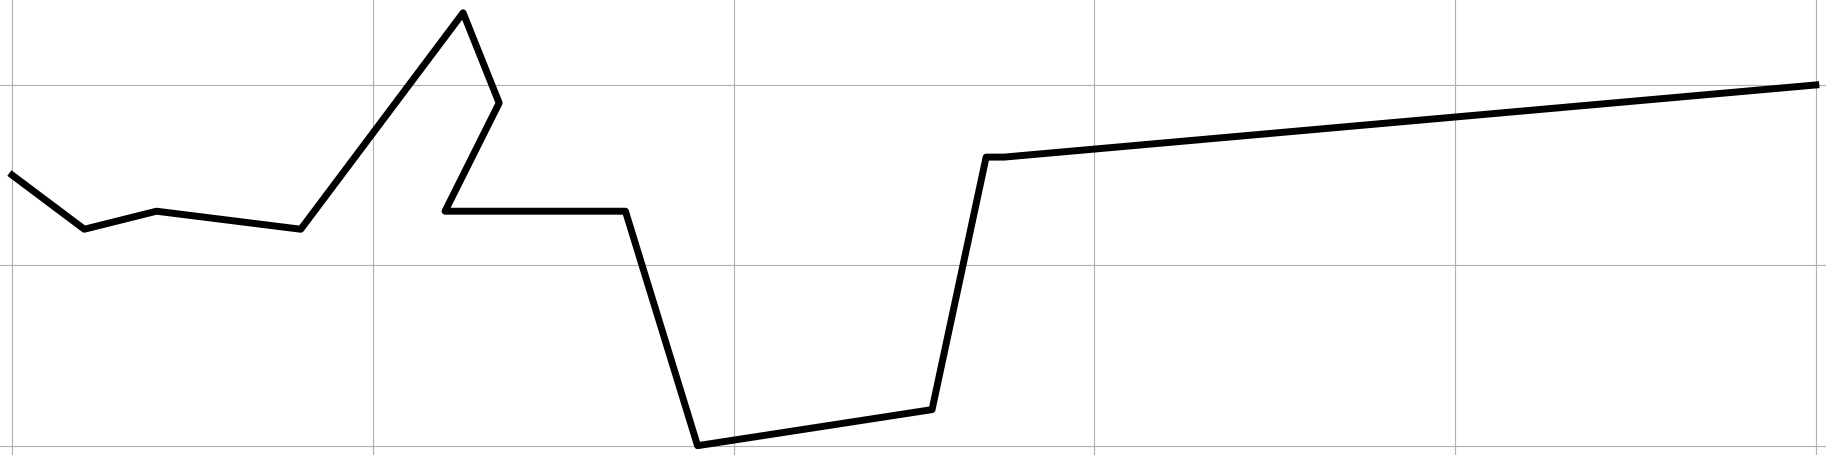
\includegraphics[width=0.8\textwidth]{raw_path_cropped.png}
		\end{figure}
		\[\Downarrow\]
		\[S = [0, 5.0, 9.1, 17.2, 32.2, 37.6, 44.3, 54.3, 67.9, 81.0, 95.4, 96.4, 141.5]\]
	\end{frame}
	
	\begin{frame}{WSPD - Algorithmus für unsere Anwendung}
		\begin{itemize}
			\item Berechnen eines \emph{(fairen) Split-Trees} $T$ aus $S$
		\end{itemize}
		\[S = [0, 5.0, 9.1, 17.2, 32.2, 37.6, 44.3, 54.3, 67.9, 81.0, 95.4, 96.4, 141.5]\]
		\[\Downarrow\]
		\begin{figure}
			\centering
			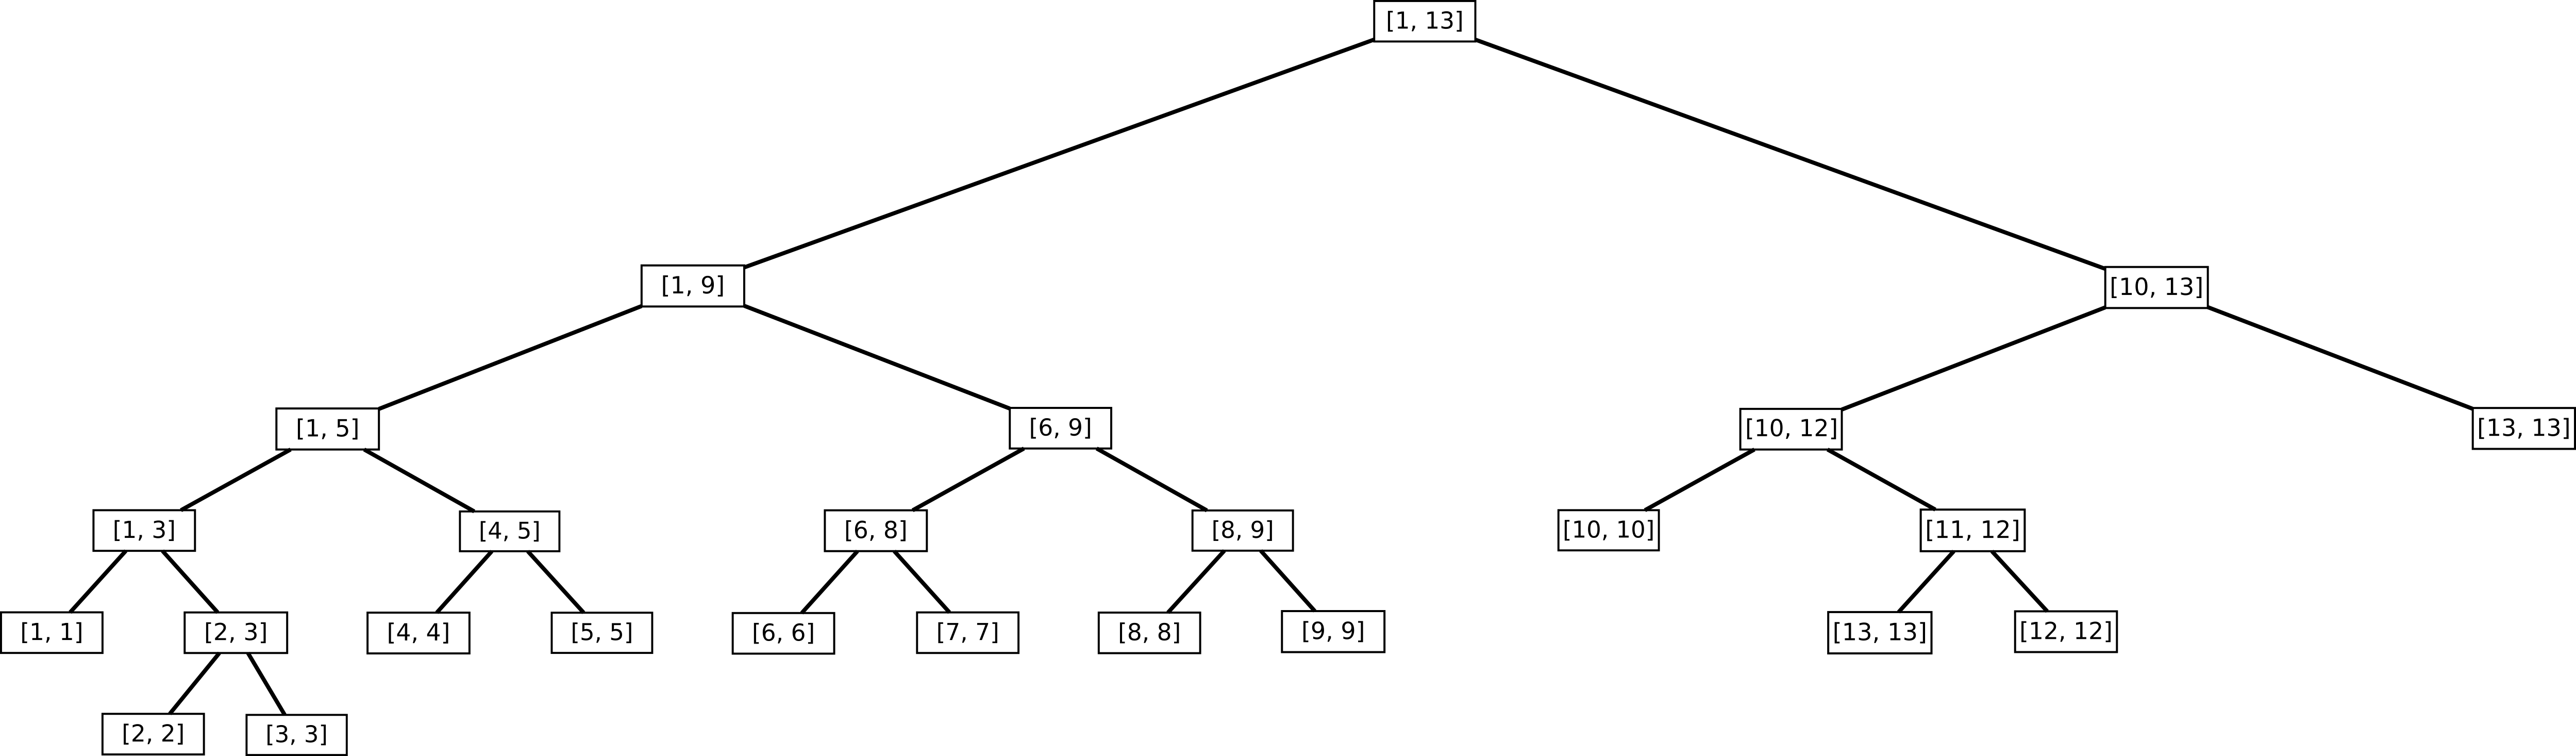
\includegraphics[width=\textwidth]{split_tree.png}
		\end{figure}
	\end{frame}
	
	\begin{frame}[t]{WSPD - Algorithmus für unsere Anwendung}
		$S = [0, 5.0, 9.1, 17.2, 32.2, 37.6, 44.3, 54.3, 67.9, 81.0, 95.4, 96.4, 141.5]$
		\begin{itemize}
			\item Berechnen einer WSPD aus dem Split-Tree $T$
		\end{itemize}
		\begin{figure}
			\centering
			\def \svgwidth{\textwidth}
			\begin{overprint}
				\onslide<1>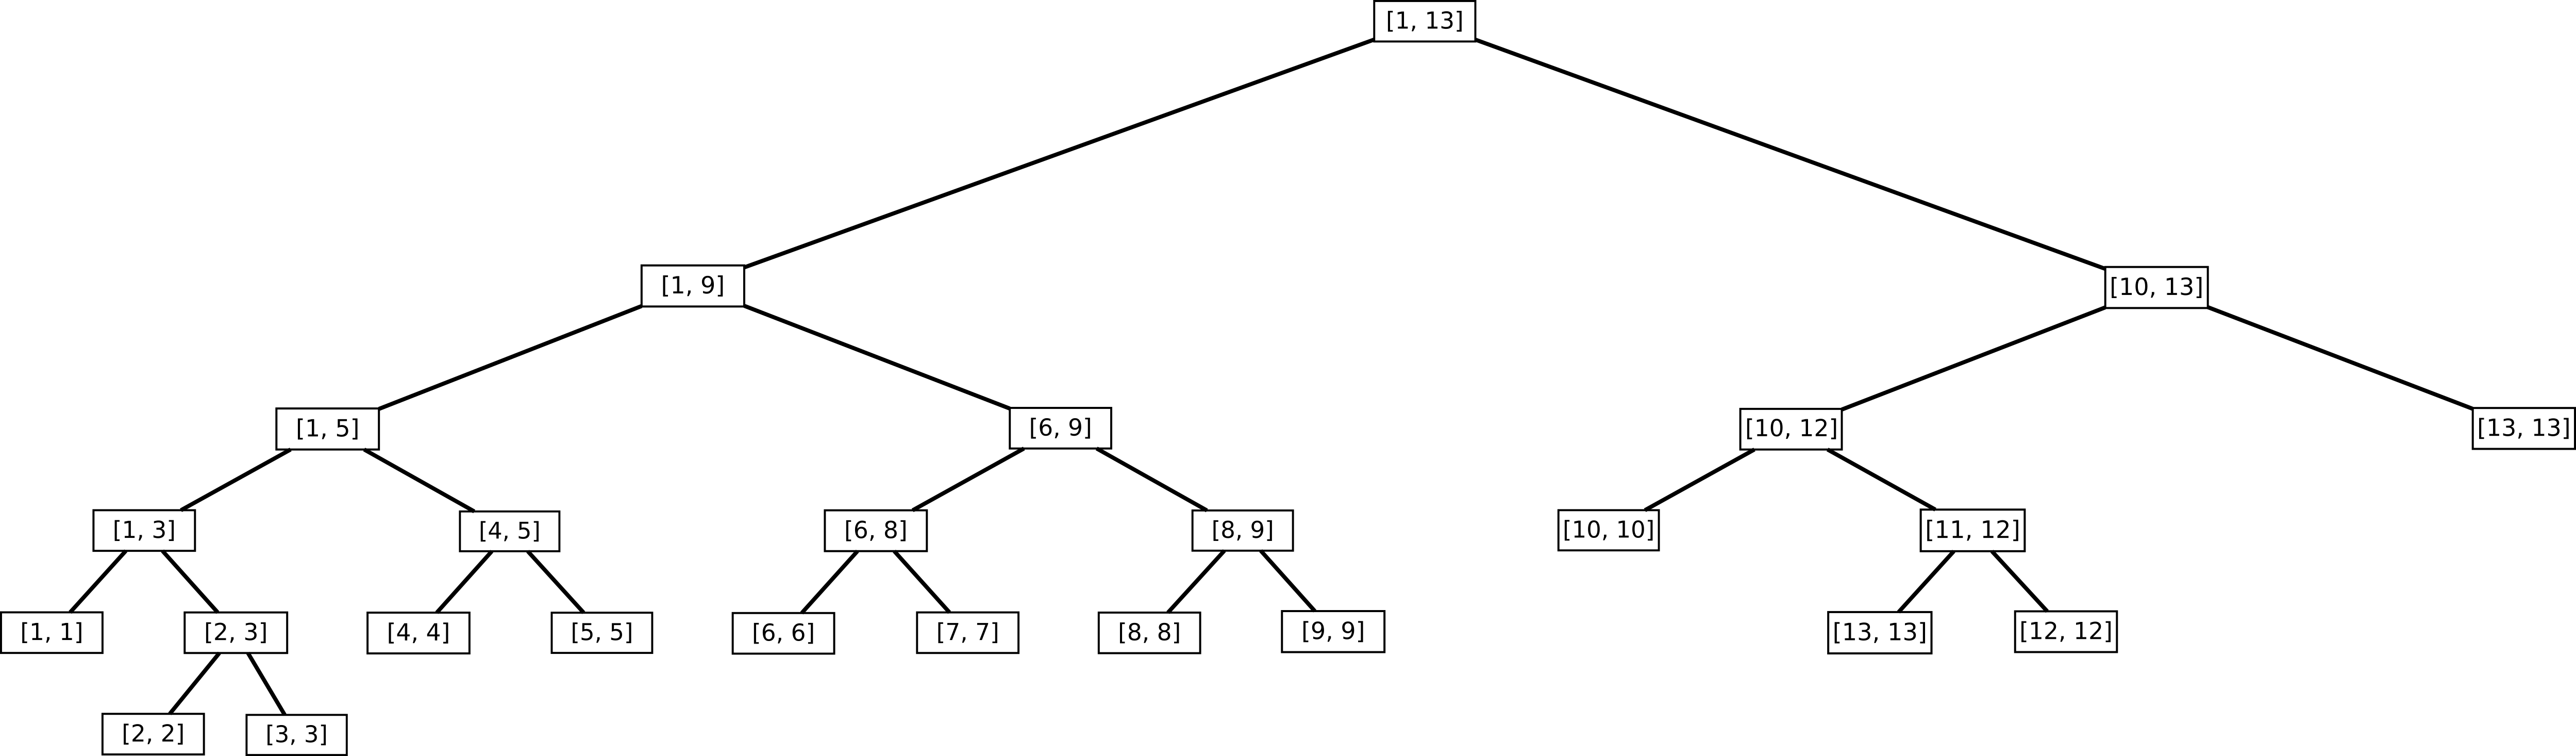
\includegraphics[width=\textwidth]{split_tree.png}
				\onslide<2->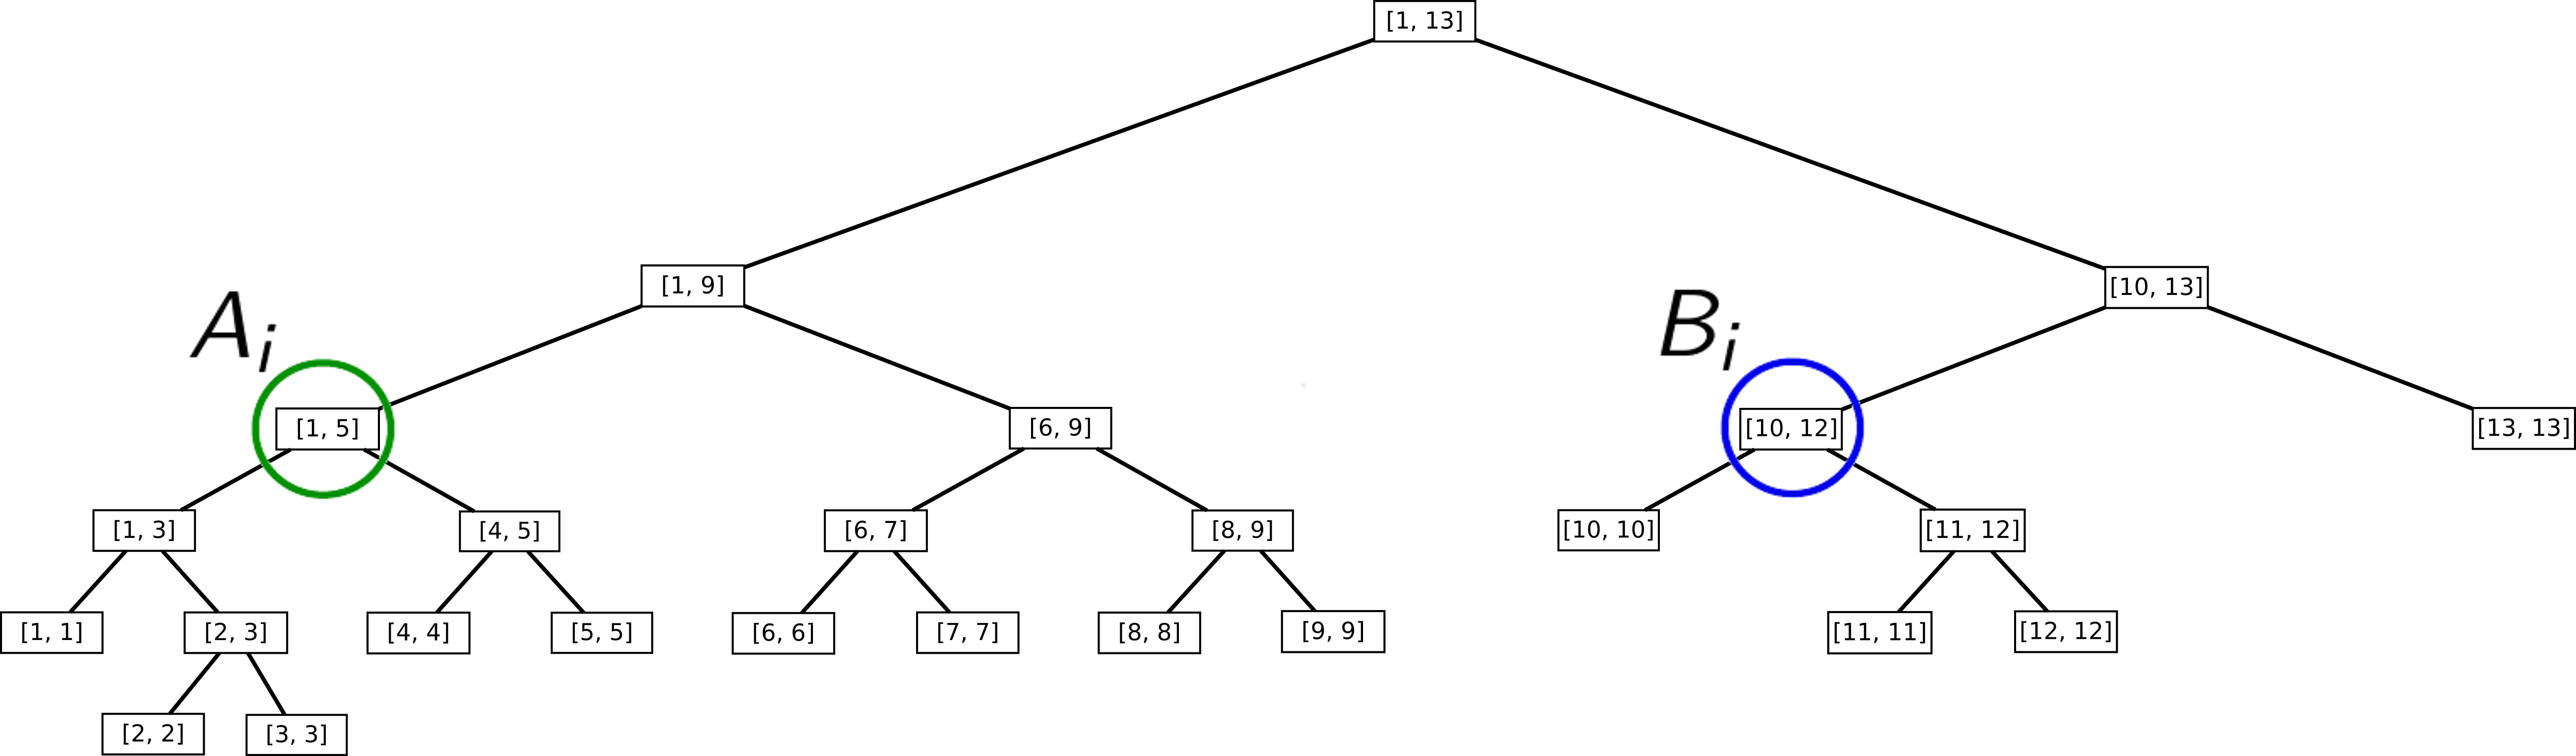
\includegraphics[width=\textwidth]{split_tree_2_wspd.png}
			\end{overprint}
			\onslide<2->\[
			R = \max(S[5]-S[1], S[12]-S[10]) = \max(32.2 - 0, 96.4 - 81) = 15.4
			\]
			\[
			S[10]- S[5] = 81 - 32.2 = 48.8 \geq 3 \cdot R = 3 \cdot 15.4
			\]
		\end{figure}

	\end{frame}

	\begin{frame}{Laufzeit}
		\begin{thm}[Callahan/Kosaraju]
			Sei $S \subset \mathbb{R}$ endlich und $n \coloneqq |S|$. Dann kann in $O(n \log n + sn)$ Zeit ein Split-Tree $T$ und eine dazugehörige WSPD $\{(A_1, B_1), (A_2, B_2), \mathellipsis, (A_m, B_m)\}$ der Größe $m = O(sn)$ berechnet werden.
		\end{thm}
	\end{frame}
	
	\subsection{Theorie}
	\begin{frame}
		Sei $0 < \epsilon < \frac{1}{3} $ und $s = \frac{12 + 24(1 + \frac{\epsilon}{3})\cdot t}{\epsilon}$.
		\begin{lemma}
	    	Seien $p, p', q, q' \in P$, sodass $\rho \coloneqq \delta(p_1, p) \in A_i$, $\rho' \coloneqq \delta(p_1, p') \in A_i$, $\varphi \coloneqq \delta(p_1, q) \in B_i$ und $\varphi' \coloneqq \delta(p_1, q') \in B_i$. Dann gilt:
	    	\begin{enumerate}
	    		\item $(p, q)$ $t$-distanzerhaltend $\Rightarrow$ $(p', q')$ $(1 + \frac{\epsilon}{3})t$-distanzerhaltend.
	    		\item $(p, q)$ $(1 + \frac{\epsilon}{3})t$-distanzerhaltend $\Rightarrow$ $(p', q')$ $(1 + \epsilon)t$-distanzerhaltend.
	    	\end{enumerate}
		\end{lemma}
		\begin{figure}
			\def \svgwidth{\textwidth}
			\onslide<2->{\input{t_epsilon_example.pdf_tex}}
		\end{figure}
	\end{frame}
	
	\begin{frame}[t]{Konstruktion eines Graphen $H$}
		\begin{block}{}
			\begin{itemize}
				\item $S = \{x_1, x_2, \mathellipsis, x_n\}$ mit $x_i = \delta(p_1, p_n)$
				\item WSPD $\{(A_1, B_1), (A_2, B_2), \mathellipsis, (A_m, B_m)\}$
			\end{itemize}
		\end{block}
		\begin{itemize}
			\item Wahl von festen Elementen $a_i \in A_i$ und $b_i \in B_i$.
			\item $\alpha_i$ und $\beta_i$ so, dass $a_i = \delta(p_1, \alpha_i)$ und $b_i = \delta(p_1, \beta_i)$.
			\item $(A_i, B_i)$ $(1 + \frac{\epsilon}{3})t$-distanzerhaltend $\Leftrightarrow$ $(\alpha_i, \beta_i)$ $(1 + \frac{\epsilon}{3})t$-distanzerhaltend
		\end{itemize}

		
		Konstruktion eines Graphen $H = (V, E)$:
		\begin{itemize}
			\item $V \coloneqq \{A_i\ |\ 1 \leq i \leq m\} \cup \{B_i\ |\ 1\leq i \leq m\}$
			\item Kanten $E$:
			\begin{enumerate}
				\item Für alle $1 \leq i \leq m$ ist $(A_i, B_i)$ genau dann eine Kante, wenn $(A_i, B_i)$ $(1 + \frac{\epsilon}{3})t$-distanzerhaltend ist und $x_n \in B_i$.
				\item Für alle $1\leq i < j \leq m$ ist $(A_i, A_j)$ genau dann eine Kante, wenn $(A_i, B_i)$ $(1 + \frac{\epsilon}{3})t$-distanzerhaltend ist und $A_j \cap B_i \neq \emptyset$.
			\end{enumerate}
		\end{itemize}
	\end{frame}
	
	\begin{frame}[t]{Approximation $\rightarrow$ $H$}
		$S = \{x_1, x_2, \mathellipsis, x_n\}$ mit $x_i = \delta(p_1, p_n)$
		\begin{thm}
			Jede $t$-distanzerhaltende Approximation $Q = (q_1, q_2, \mathellipsis, q_k)$ von $P$ entspricht einem Pfad $R$ der Länge $k$ in H von einer Menge $A_i$, die $x_1$ enthält, zu einer Menge $B_j$, die $x_n$ enthält.
		\end{thm}
		\textit{Beweis.} Induktive Konversion von $Q$ zu $R$.
		
		Sei $y_i$ das Element der Menge $S$, für das $y_i = \delta(p_1, q_i)$ gilt. 
		\begin{itemize}
			\item Da $q_1 = p_1$, ist $y_1 = x_1$.
			Sei $i_1$ der Index, für den $y_1 \in A_{i_1}$ und $y_2 \in B_{i_1}$ ist. 
			
			Dann wählen wir $A_{i_1}$ als ersten Knoten des Pfades $R$.
		\end{itemize}
	\end{frame}
	
	\begin{frame}
		$S = \{x_1, x_2, \mathellipsis, x_n\}$ mit $x_i = \delta(p_1, p_n)$
		$y_i = \delta(p_1, q_i)$ 
		
		\begin{itemize}
			\item asdf
		\end{itemize}
	
	\end{frame}
	
	\begin{frame}{$H$ $\rightarrow$ Approximation}
		\begin{thm}
			Jeder Pfad $R = (A_{i_1}, \mathellipsis, A_{i_{k-1}}, B_{i_{k-1}})$ in $H$ mit $x_1 \in A_{i_1}$ und $x_n \in B_{i_{k-1}}$ entspricht einer $(1+\epsilon)t$-distanzerhaltenden Approximation $Q$ von $P$, die $k$ Knoten besitzt.
		\end{thm}
		\textit{Beweis.}
		Sei $y_i$ das Element der Menge $S$, für das $y_i = \delta(p_1, q_i)$ gilt.
		\begin{itemize}
			\item $q_1 \coloneqq p_1$
		\end{itemize}
	\end{frame}
	
	\begin{frame}[t]
		\begin{block}{Wiederholung}
			\begin{itemize}
				\item $y_i = \delta(p_1, q_i)$
				\item Für alle $1\leq i < j \leq m$ ist $(A_i, A_j)$ genau dann eine Kante, wenn $(A_i, B_i)$ $(1 + \frac{\epsilon}{3})t$-distanzerhaltend ist und $A_j \cap B_i \neq \emptyset$.
			\end{itemize}
		\end{block}
		
		
		\vspace{10px}
		\begin{itemize}
			\item Annahme: für ein $l$ mit $1 \leq l < k-1$ wurde der Teilpfad $(A_{i_1}, \mathellipsis, A_{i_l})$ bereits in den Kantenzug $(q_1, \mathellipsis, q_l)$ umgewandelt, sodass für alle $1 < j \leq l$ $y_j \in A_{i_j} \cap B_{i_{j-1}}$.  
			Wir betrachten die Kante $(A_{i_l}, A_{i_{l+1}})$.
			\begin{itemize}
				\item Es gibt ein $y \in A_{i_{l+1}} \cap B_{i_l}$.
				\item $q_{l+1}$ ist der Knoten $\gamma$ von $P$, für den $y = \delta(p_1, \gamma)$ gilt 
%				und erhalten $(q_1, \mathellipsis, q_l, q_{l+1})$.
			\end{itemize}
			\item Annahme: $(A_{i_1}, \mathellipsis, A_{i_k-1})$ wurde bereits zu $(q_1, \mathellipsis, q_{k-1})$ umgewandelt haben. 
			Nach Voraussetzung ist $x_n \in B_{k-1}$. 
			
			$\Rightarrow q_k \coloneqq p_n$. 
		\end{itemize}
	\end{frame}
	
	\begin{frame}
		\begin{description}
			\item[Bereits gezeigt: ] Umwandlung in Kantenzug $Q = (q_1, q_2, \mathellipsis, q_k)$.
			\item[Noch zu zeigen: ] $Q$ ist $(1 + \epsilon)t$-distanzerhaltend.
		\end{description}
		
		Sei $1 \leq i < k$.
		
		\begin{itemize}
			\item $(q_i, q_{i+1})$ ist durch Umwandlung aus $(A_i, A_{i+1})$ entstanden, wobei $q_i \in A_i$ und $q_{i+1} \in B_i\ (\cap\ A_{i+1})$.
			
			\item Nach Konstruktion von $H$: $(A_i, B_i)$ ist $(1 + \frac{\epsilon}{3})t$-distanzerhaltend.
			
			\item Also ist $(\alpha_i, \beta_i)$ $(1 + \frac{\epsilon}{3})t$-distanzerhaltend.
			
			\item $\stackrel{Lemma}{\Rightarrow}$ $(q_i, q_{i+1})$ ist $(1 + \epsilon)t$-distanzerhaltend.
		\end{itemize}
		
	\end{frame}
	
	\subsection{Algorithmus}
	\begin{frame}{Algorithmus}
		\begin{description}
			\item[Schritt 1:] Berechnen von $S = (x_1, \mathellipsis, x_n)$ mit $x_i = \delta(p_1, p_i)$
			\item[Schritt 2:] Berechnen des Split-Trees $T$ und einer WSPD $\{(A_1, B_1), (A_2, B_2), \mathellipsis, (A_m, B_m)\}$ mit der Trennungsrate $s = \frac{12 + 24(1 + \frac{\epsilon}{3})t}{\epsilon}$. 
%			Nehme wieder o.B.d.A. an, dass für alle $1 \leq i \leq m'$ alle Elemente aus $A_i$ kleiner sind als alle aus $B_i$.
			\item[Schritt 3:] Wählen von $a_i \in A_i$, $b_i \in B_i$, $\alpha_i$ und  $\beta_i$ die Knoten von $P$ sind, für die $a_i = \delta(p_1, \alpha_i)$ und $b_i = \delta(p_1, \beta_i)$. 
			Falls $(\alpha_i, \beta_i)$ nicht $(1+\frac{\epsilon}{3})t$-distanzerhaltend ist, verwirf das korrespondierende Tupel $(A_i, B_i)$, ansonsten behalte es.
		\end{description}
	\end{frame} 
	
	\begin{frame}[t]{Modifizierte Breitensuche}
		Sei $k$ Knoten im Baum. 
		
		$d[k]$: Distanz von $k$ zum Startknoten
		\begin{figure}
			\begin{overprint}
				\onslide<1>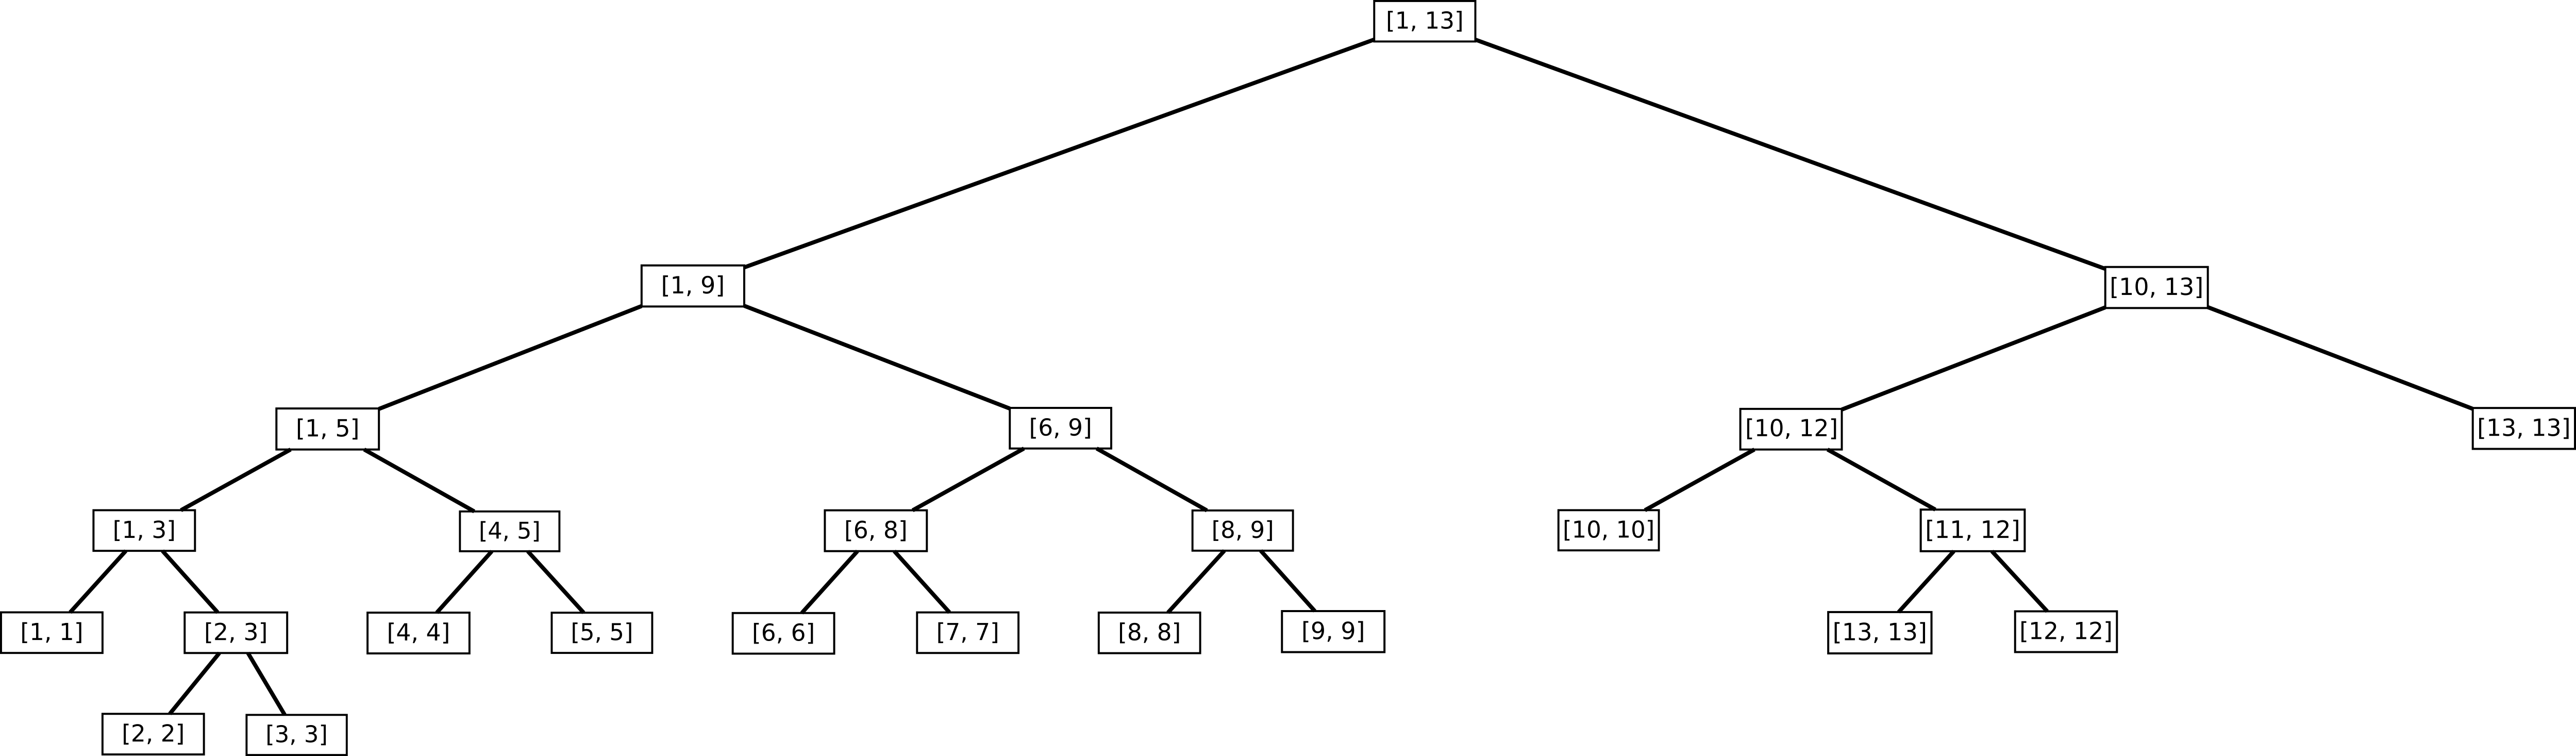
\includegraphics[width=\textwidth]{split_tree.png}
				\onslide<2>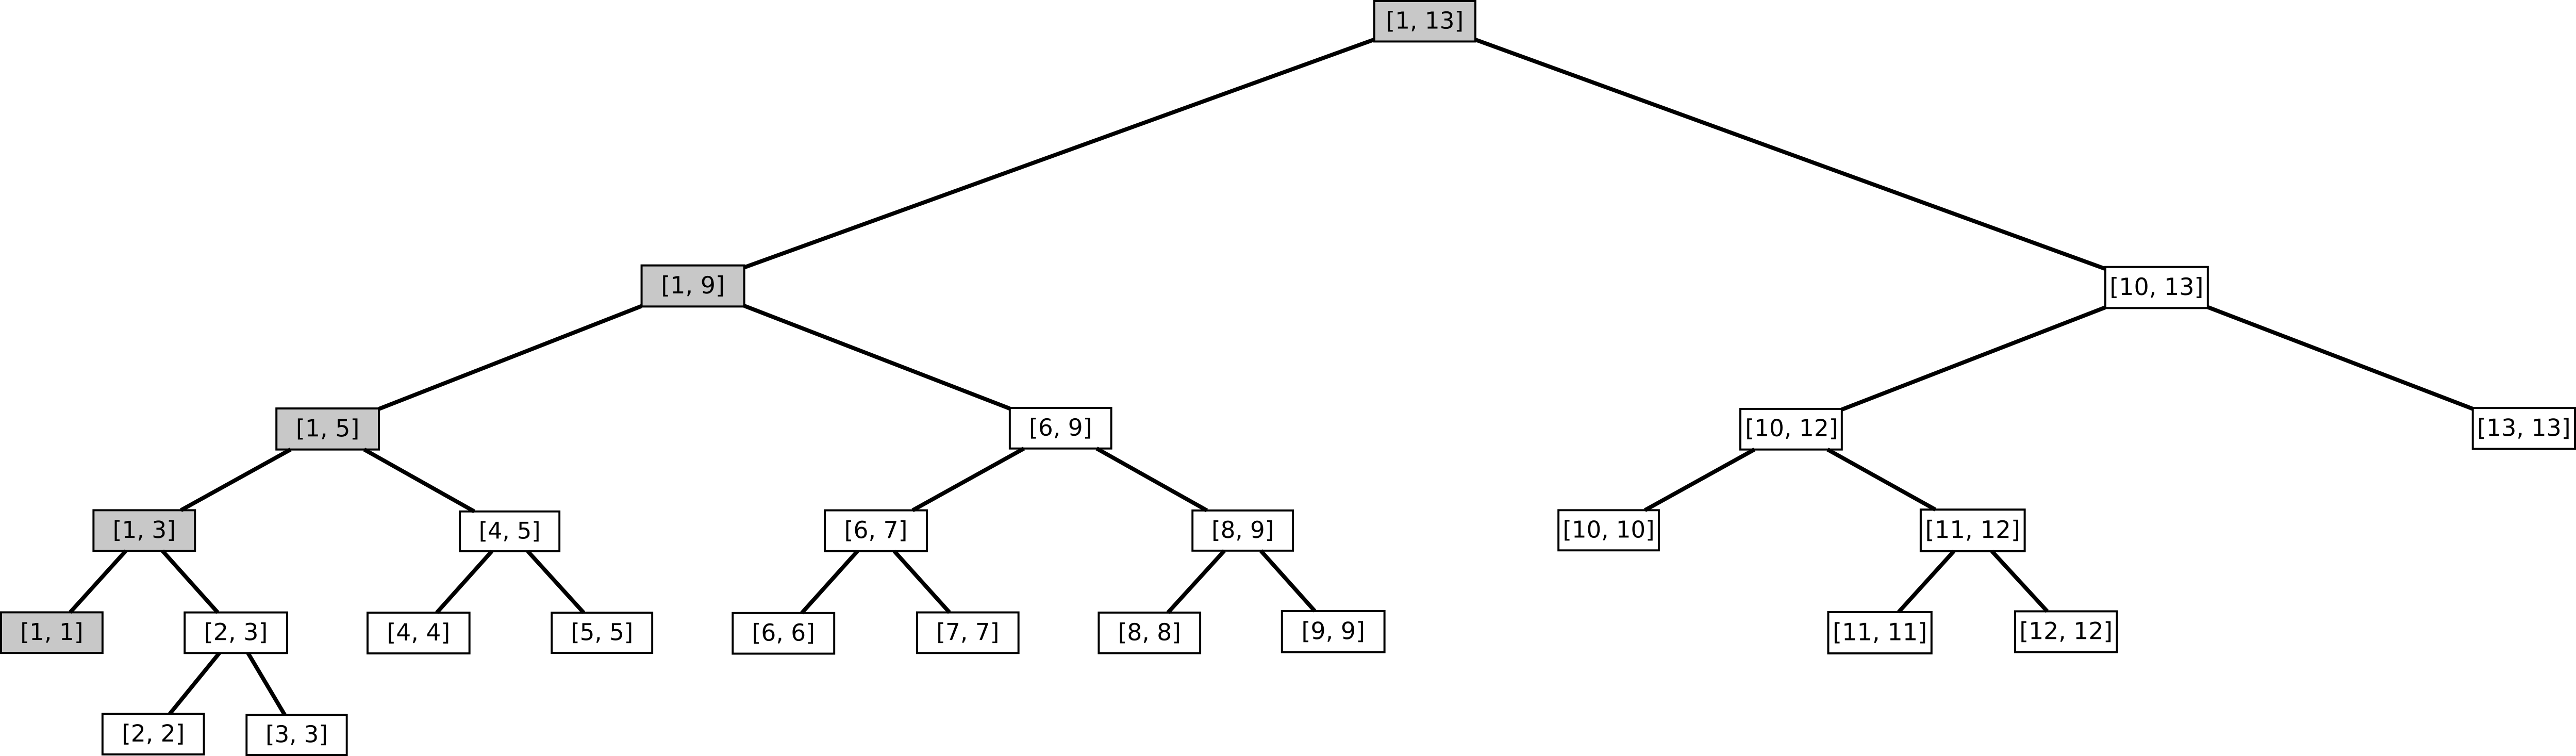
\includegraphics[width=\textwidth]{bfs_step1.png}
				\onslide<3>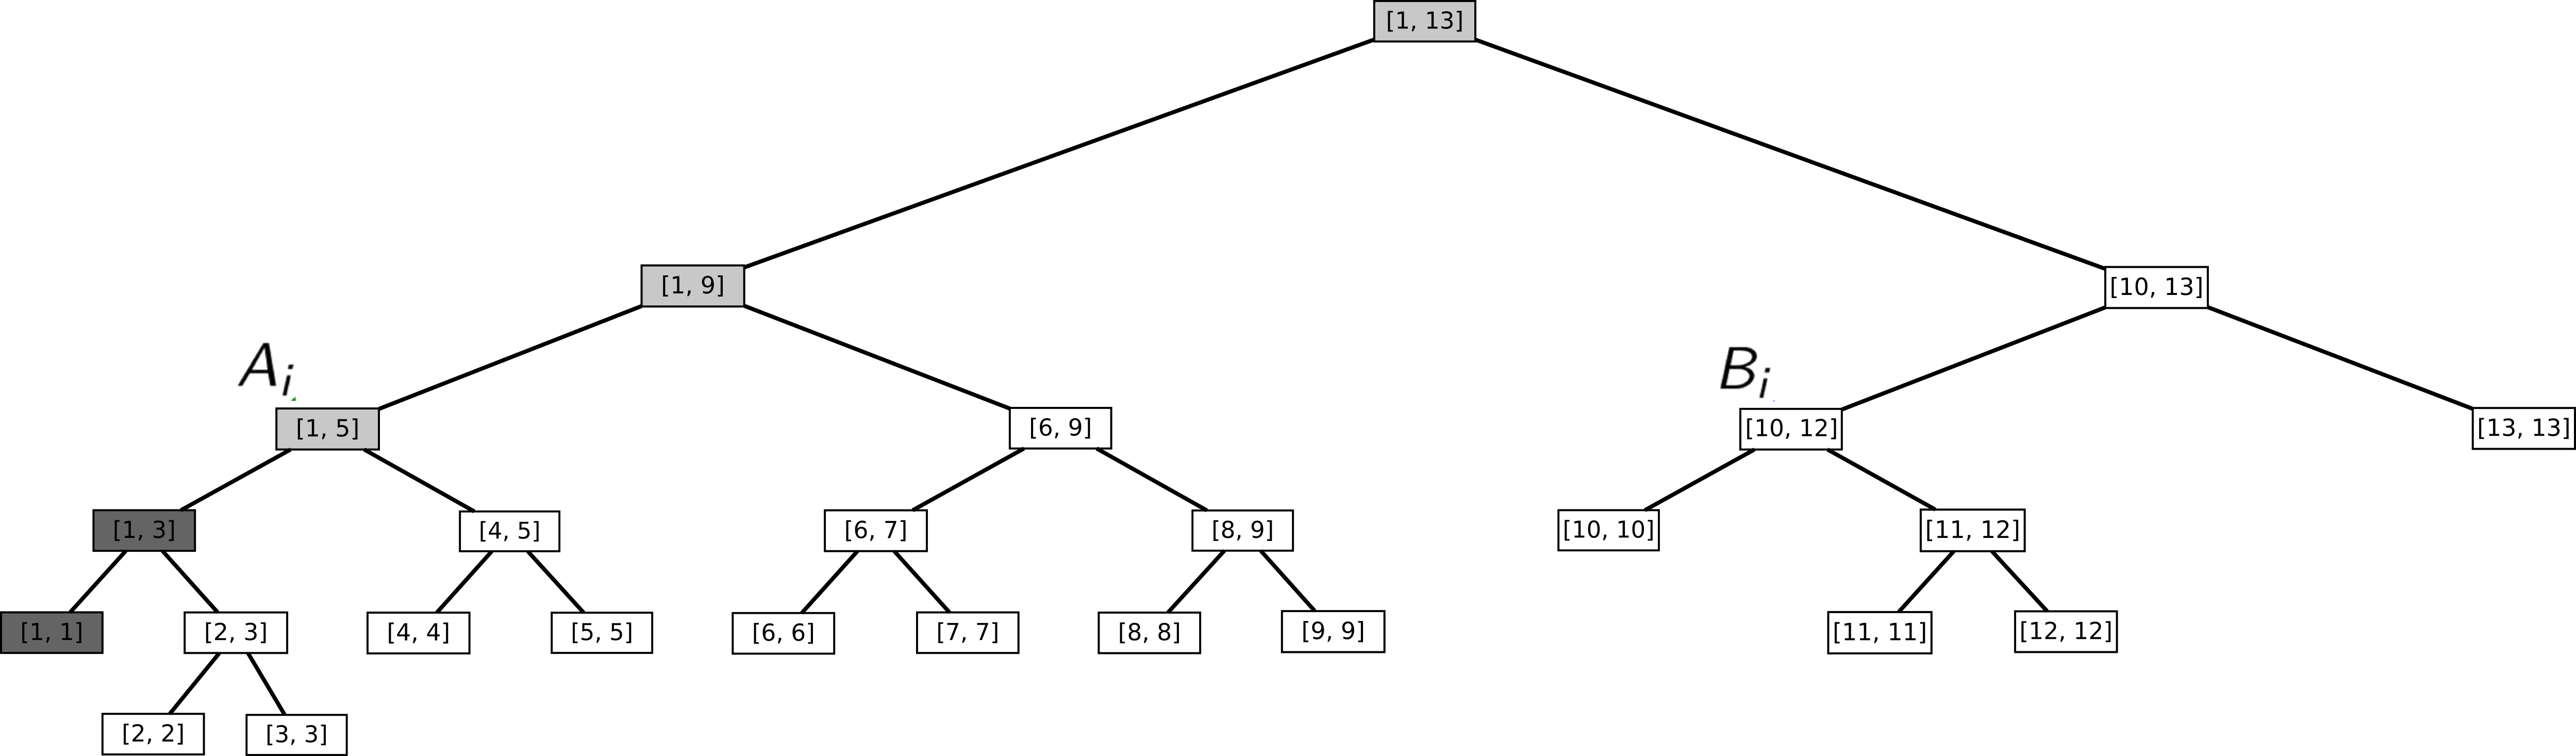
\includegraphics[width=\textwidth]{bfs_step2.png}
				\onslide<4>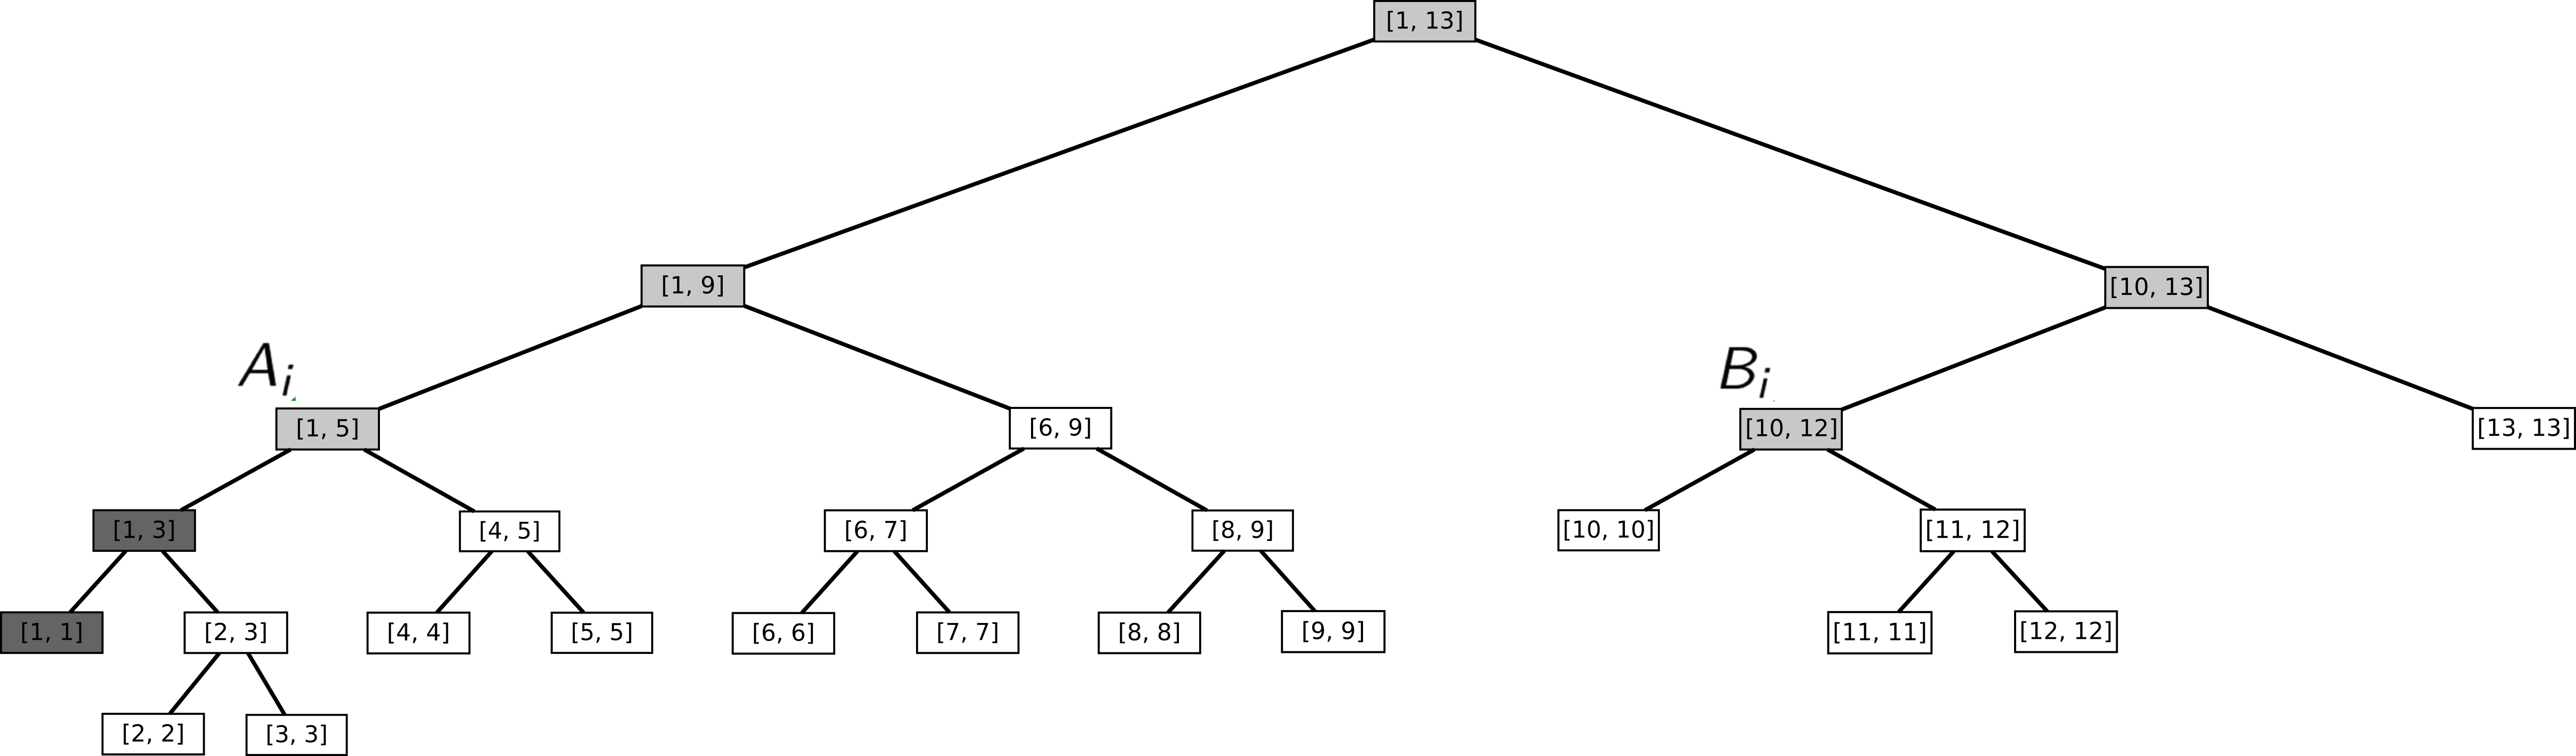
\includegraphics[width=\textwidth]{bfs_step3.png}
				\onslide<5>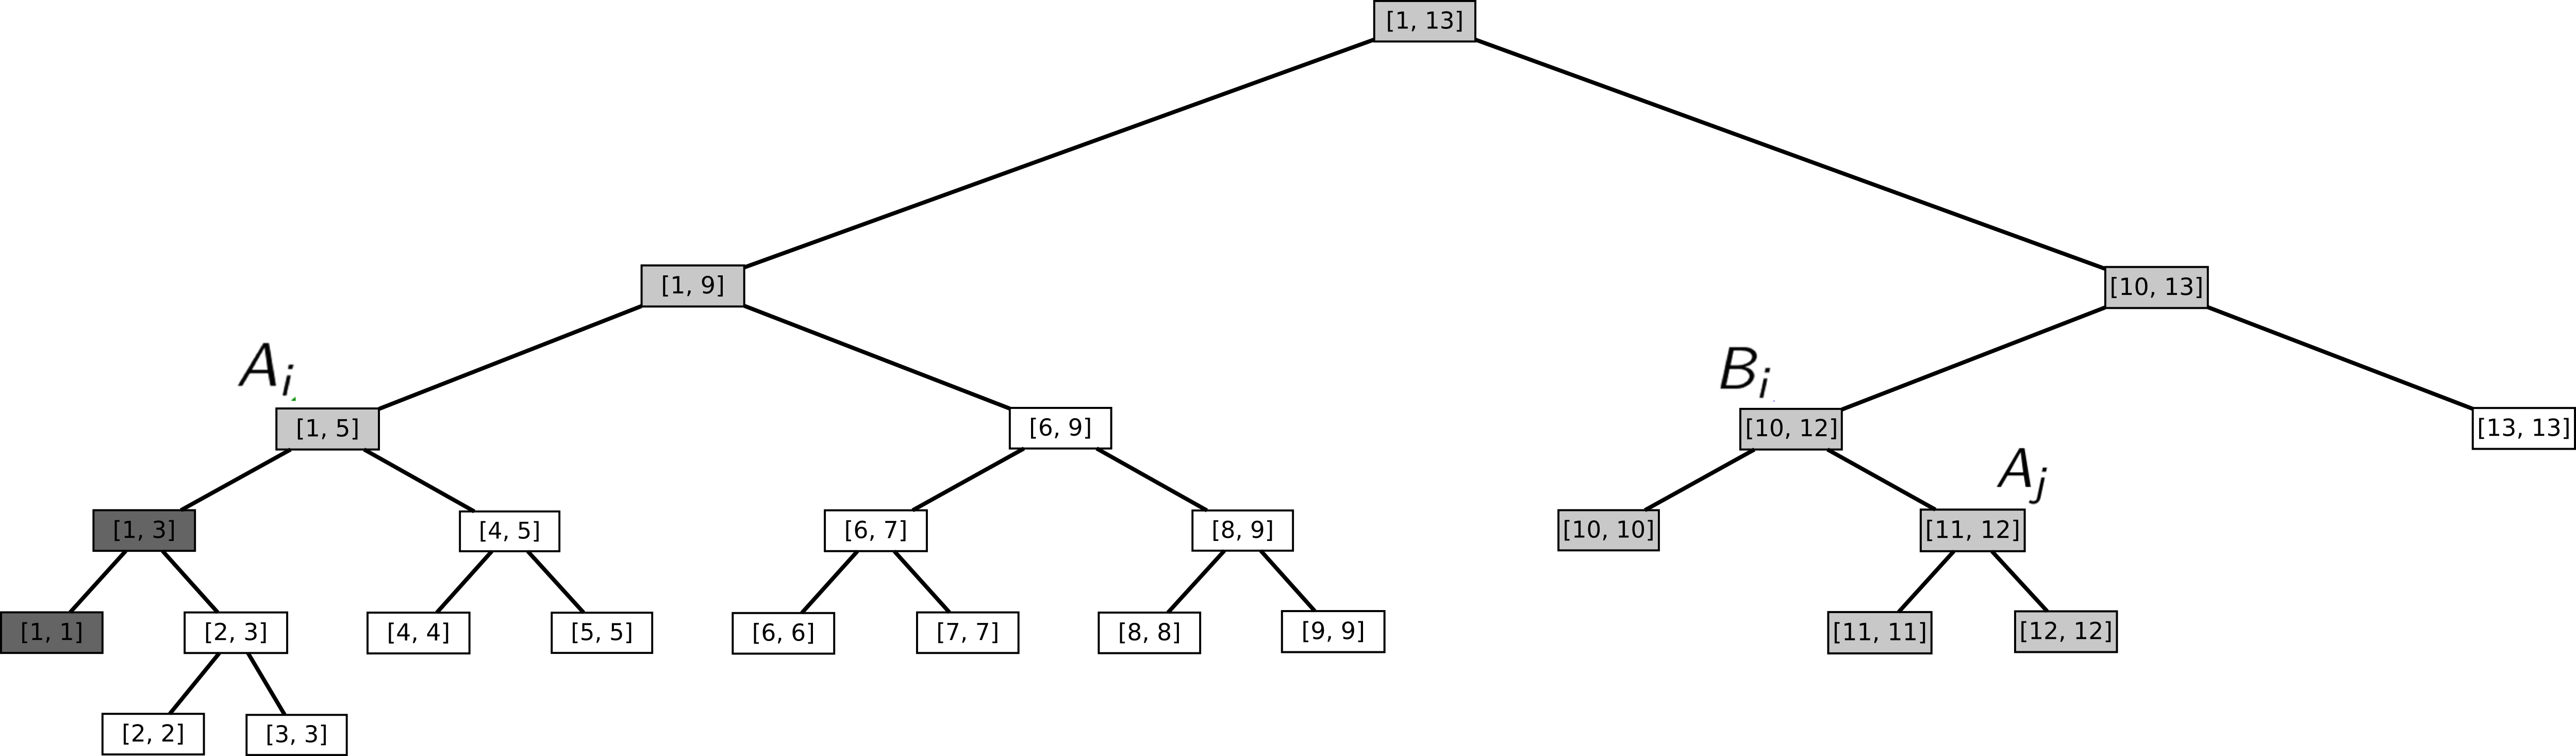
\includegraphics[width=\textwidth]{bfs_step4.png}
				\onslide<6>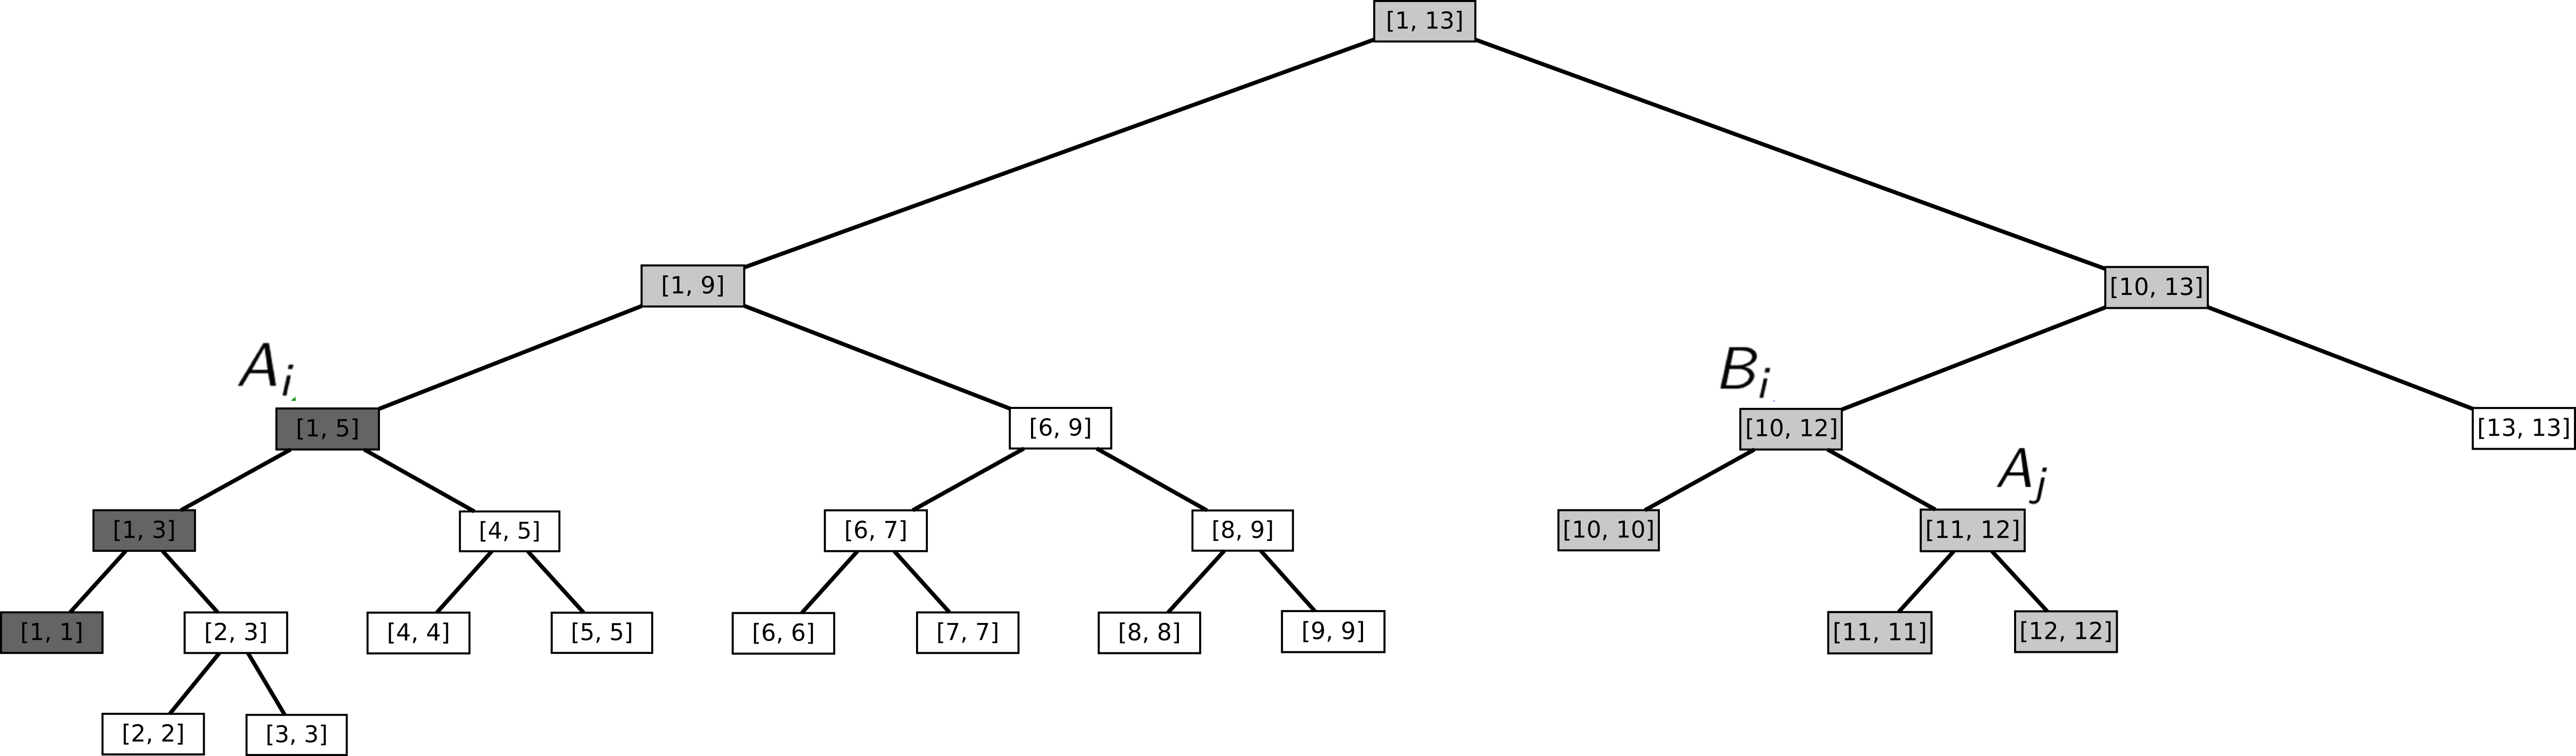
\includegraphics[width=\textwidth]{bfs_step5.png}
			\end{overprint}
		\end{figure}
		
		\begin{overprint}
			
			\onslide<2> \centering Falls A-Knoten $k$, $d[k] = 0$
			\onslide<5> \centering$d[A_j] = d[A_i] + 1$
				
				\centering Füge $A_j$ zur Warteschlange hinzu
			
		\end{overprint}
	\end{frame}
	
	\begin{frame}{Algorithmus}
			\begin{description}
				\item[Schritt 1:] Berechnen von $S = (x_1, \mathellipsis, x_n)$ mit $x_i = \delta(p_1, p_i)$
				\item[Schritt 2:] Berechnen des Split-Trees $T$ und einer WSPD $\{(A_1, B_1), (A_2, B_2), \mathellipsis, (A_m, B_m)\}$ mit der Trennungsrate $s = \frac{12 + 24(1 + \frac{\epsilon}{3})t}{\epsilon}$. 
				%			Nehme wieder o.B.d.A. an, dass für alle $1 \leq i \leq m'$ alle Elemente aus $A_i$ kleiner sind als alle aus $B_i$.
				\item[Schritt 3:] Wählen von $a_i \in A_i$, $b_i \in B_i$, $\alpha_i$ und  $\beta_i$ die Knoten von $P$ sind, für die $a_i = \delta(p_1, \alpha_i)$ und $b_i = \delta(p_1, \beta_i)$. 
				Falls $(\alpha_i, \beta_i)$ nicht $(1+\frac{\epsilon}{3})t$-distanzerhaltend ist, verwirf das korrespondierende Tupel $(A_i, B_i)$, ansonsten behalte es.
				\item<2->[Schritt 4:] Ausführen der modifizierte Breitensuche im Split-Tree $T$ durch.
				\item<3->[Schritt 5:] Umwandeln des erhaltenen Pfades $(A_{i_1}, \mathellipsis, A_{i_{k-1}}, B_{i_{k-1}})$ zu einer Approximation von $P$
			\end{description}
	\end{frame}
	
	\begin{frame}{Laufzeit}
		\centering
		$s = \frac{12 + 24(1 + \frac{\epsilon}{3})t}{\epsilon}$ $\Rightarrow$ $O(sn) = O(\frac{t}{\epsilon}n)$
		\begin{columns}
			\begin{column}{0.6\textwidth}
				\begin{description}
					\item[Schritt 1:]<1-> Berechnen von $S$
					\item[Schritt 2:]<2-> Berechnen der WSPD
					\item[Schritt 3:]<3-> Aussortieren der WSPD
					\item[Schritt 4:]<4-> Modifizierte Breitensuche
					\item[Schritt 5:]<5-> Umwandeln in Approximation
				\end{description}
			\end{column}
			\begin{column}{0.6\textwidth}
				\begin{description}
					\item[]<1-> $O(n)$
					\item[]<2-> $O(n \log n + \frac{t}{\epsilon}n)$
					\item[]<3-> $O(\frac{t}{\epsilon}n)$
					\item[]<4-> $O(\frac{t}{\epsilon}n)$
					\item[]<5-> $O(\frac{t}{\epsilon}n)$
				\end{description}
			\end{column}
		\end{columns}
	\end{frame}
	
	\begin{frame}
		\begin{thm}
		   	Sei $P = (p_1, p_2, \mathellipsis, p_n)$ ein Kantenzug in $\mathbb{R}^d$, sei $t \geq 1$ und $0 < \epsilon < \frac{1}{3}$ und sei $\kappa$ die Knotenzahl der minimalen t-distanzerhaltenden Approximationen von $P$. Dann können wir in $O(n \log n + \frac{t}{\epsilon}n)$ eine $(1 + \epsilon)t$-distanzerhaltende Approximation $Q$ von $P$ mit maximal $\kappa$ Knoten berechnen.
		\end{thm}
	\end{frame}
\end{document}